\documentclass[zihao=-4]{ctexart}
\usepackage[normalem]{ulem}
\useunder{\uline}{\ul}{}
%********************导言区宏包引入********************
\usepackage{xeCJK}
\usepackage{amssymb}
\usepackage{amsmath}
\usepackage{listings} %代码
\usepackage{graphicx}
\usepackage{multicol} %回车换段
\usepackage{xcolor}
\usepackage{geometry} %页面设置
\usepackage{fontspec}
\usepackage{setspace}
\usepackage{times}
\usepackage{fancyhdr} %页眉页脚
\pagestyle{fancy}
\usepackage{float} %表格位置
\usepackage{titlesec} %设置
\usepackage{titletoc}
\usepackage{ctex}
\usepackage{gbt7714}    %控制参考文献格式为国标
\usepackage{multirow}
\usepackage{booktabs}   %表格相关
\usepackage{setspace}   %设置行距
\usepackage{caption} %caption
\usepackage{subcaption} %子图的caption
\usepackage{changepage} %左右缩进


\graphicspath{ {pictures/} }
\let\algorithm\relax
\let\endalgorithm\relax
\usepackage[ruled,vlined]{algorithm2e}%[ruled,vlined]{
\usepackage{algpseudocode}
\renewcommand{\algorithmicrequire}{\textbf{Input:}} 
\renewcommand{\algorithmicensure}{\textbf{Output:}}
%\renewcommand\thepage{\zihao{-5} ~\arabic{page}~}%页码字号

%定义两个arg
\DeclareMathOperator*{\argmax}{arg\,max}
\DeclareMathOperator*{\argmin}{arg\,min}
\DeclareCaptionLabelSeparator{mysep}{\space\space}  %自定义caption格式
\captionsetup[figure]{font={small}, labelfont=bf, labelsep=mysep, textfont=bf}   %图片caption格式
\captionsetup[table]{font={small}, labelfont=bf, labelsep=mysep, textfont={bf}}   %表格caption格式
\bibliographystyle{gbt7714-numerical} %修改了title斜体内容

%********************导言区宏包引入********************
%********************第三方字体引入********************
%\setCJKmainfont[Path=fonts/,BoldFont=simhei.ttf,ItalicFont=simkai.ttf,SlantedFont=simfang.ttf]{simsun.ttc}
%中文字体涵盖黑体、宋体、楷体、仿宋
\setmainfont[Path=fonts/, 
BoldFont = times-new-roman-bold.ttf,
ItalicFont = times-new-roman-italic.ttf,
BoldItalicFont = times-new-roman-bold-italic.ttf
]{times-new-roman.ttf}
\setmonofont[Path=fonts/]{Courier New.ttf}
\setCJKfamilyfont{hwzs}[Path=fonts/]{STKzhongsong.ttf}%使用STZhogsong华文中宋字体
\newcommand{\zhongsong}{\CJKfamily{hwzs}}
\setCJKfamilyfont{hwxw}[Path=fonts/]{STKxinwei.ttf} % XSP 2023/3/3:
\newcommand{\xinwei}{\CJKfamily{hwxw}}              %  使用STZxinwei华文新魏字体.

%********************第三方字体引入********************

%********************代码段设置********************
% by yjw
% \texttt 用于行内代码,等宽字体,不知道让不让用
\usepackage{listings} % 用于代码排版
\usepackage{xcolor} % 用于代码高亮

% 定义代码块样式
\lstdefinestyle{codeblock}{
    backgroundcolor=\color{white},    % 背景颜色
    basicstyle=\ttfamily\small,       % 设置字体样式
    breakatwhitespace=false,          % 是否只在空白处自动断行
    breaklines=true,                  % 自动断行
    captionpos=b,                     % 标题位置
    commentstyle=\color{gray},       % 注释风格
    frame=single,                     % 单框
    keepspaces=true,                  % 保持空格
    keywordstyle=\color{blue},        % 关键字风格
    numbers=left,                     % 行号位置
    numbersep=8pt,                    % 行号与代码的距离
    numberstyle=\tiny\color{gray},    % 行号样式
    rulecolor=\color{black},          % 框架颜色
    showspaces=false,                 % 不显示空格
    showstringspaces=false,           % 字符串中不显示空格
    showtabs=false,                   % 不显示制表符
    stepnumber=1,                     % 步长
    stringstyle=\color{orange},       % 字符串风格
    tabsize=2,                        % 制表符占用空格数
    xleftmargin=\parindent,           % 左边距
    framexleftmargin=12pt,             % 框架左边距,增加些许间距以包含行号
}
\lstset{style=codeblock}

\usepackage{hyperref} %超链接支持
%********************代码段设置********************

%********************中文字号设置********************
%\newcommand{\chuhao}{\fontsize{42pt}{\baselineskip}\selectfont}
\newcommand{\chuhao}{\fontsize{42pt}{0}}
\newcommand{\xiaochu}{\fontsize{36pt}{0}}
\newcommand{\yihao}{\fontsize{28pt}{0}}
\newcommand{\erhao}{\fontsize{21pt}{0}}
\newcommand{\xiaoer}{\fontsize{18pt}{0}}
\newcommand{\sanhao}{\fontsize{16pt}{0}}
\newcommand{\sihao}{\fontsize{14pt}{0}}
\newcommand{\xiaosi}{\fontsize{12pt}{0}}
\newcommand{\wuhao}{\fontsize{10.5pt}{0}}
\newcommand{\xiaowu}{\fontsize{9pt}{0}}
\newcommand{\liuhao}{\fontsize{8pt}{0}}
\newcommand{\qihao}{\fontsize{5.25pt}{0}}
%********************中文字号设置********************


%********************页边距设置********************
\geometry{left=3cm,right=2cm,top=2.5cm,bottom=2.5cm}
\geometry{a4paper} % xsp 2023/3/7: 调整纸张大小为A4
%********************页边距设置********************

%********************段间距设置********************
\newcommand{\setParDis}{\setlength {\parskip} {0pt} }
%请在每部分使用这个
%********************段间距设置********************

%********************子文件导入区域****************
% 用于仅编译部分导入文件
% \includeonly{subtexs/ros_background, }

\begin{document}
%********************页眉页脚设置********************
\lhead{}%设置左页眉为空
\rhead{}%设置左页眉为空
\setlength{\headwidth}{\textwidth}% 2023/3/3 XSP: 页眉长度适应文本
%********************页眉页脚设置********************


%********************标题格式设置********************

%\setcounter{secnumdepth}{0}%该命令取消了章标题前数字label

\CTEXsetup[name={,、},number={\chinese{section}}]{section}
\CTEXsetup[name={(,)},number={\chinese{subsection}}]{subsection}
\CTEXsetup[name={,.},number={\arabic{subsubsection}}]{subsubsection}% 不加会导致目录格式错误
% 设置subsubsection等格式
% \titleformat{\section}[block]{\sanhao\bfseries\centering}{\chinese{section}、}{0pt}{}[]
% \titleformat{\subsection}[block]{\sihao\bfseries}{(\chinese{subsection})}{0pt}{}[]
% \titleformat{\subsubsection}[block]{\xiaosi\bfseries}{\arabic{subsubsection}、}{0pt}{}[]
\titleformat{\section}[block]{\sanhao\heiti\centering}{\chinese{section}、}{0pt}{}[]    % XSP 2023/3/3:
\titleformat{\subsection}[block]{\sihao\heiti}{(\chinese{subsection})}{0pt}{}[]       %   将正文标题字体由加粗
\titleformat{\subsubsection}[block]{\xiaosi\heiti}{\arabic{subsubsection}.}{0pt}{}[]   % 修改为黑体。
\titlespacing{\section}{0pt}{25pt}{12pt}
\titlespacing{\subsection}{0pt}{7pt}{7pt}
\titlespacing{\subsubsection}{0pt}{5pt}{4pt}

\titlecontents{section}[1.6em]{\addvspace{2pt}\filright}
{\contentspush{\thecontentslabel\hspace{0.8em}}}
{}{\titlerule*[8pt]{.}\contentspage}

\titlecontents{subsection}[3.2em]{\addvspace{2pt}\filright}
{\contentspush{\thecontentslabel\hspace{0.8em}}}
{}{\titlerule*[8pt]{.}\contentspage}

\titlecontents{subsubsection}[6.4em]{\addvspace{2pt}\filright}
{\contentspush{\thecontentslabel\hspace{0.8em}}}
{}{\titlerule*[8pt]{.}\contentspage}
%********************标题格式设置********************

%\setcounter{section}{-3}  %标题计数器
%\stepcounter{section}

%*******************行间距段前段后*******************
\linespread{1.8}
%行间距为实际行间距乘以1.2,如此处实际为1.5倍行距
\setlength{\parskip}{0.5\baselineskip}
%*******************行间距段前段后*******************



%********************封面部分********************
%
%     论文题目:应准确、鲜明、简洁,能概括整个论文中最主要和最重要的内容。
% 题目不超过20个中文字,若语意未尽,可用副标题补充说明。副标题应处于从属
% 地位,一般可在题目的下一行用破折号“——”引出。论文题目应避免使用不常用缩
% 略词、首字母缩写字、字符、代号和公式等。
%
\def\Fengru{第三十四届“冯如杯”竞赛主赛道}
\leftline{
\includegraphics[scale=1]{pictures/xiaohui.png}} % XSP 2023/3/3: 取消校徽段首缩进
%格式控制部分
% \par \  
% \par \
% \par \
\vspace{32pt}
\begin{center}

\includegraphics[height=2.25cm, width=12.78cm, scale=1]{pictures/xiaoming.png}
\end{center}
%格式控制部分
\vspace{12pt}

\begin{spacing}{3}
    % \erhao
    \begin{center}
      {
        \fontsize{22pt}{3}\selectfont
        \zhongsong{\Fengru 项目论文Latex模板} %黑体这样调用,其余字体同理
      } 
        % \zhongsong{“冯如杯”竞赛主赛道项目是什么}
    \end{center}
    \rightline{\xinwei\sanhao{——基于 Latex 的论文模板}} % XSP 2023/3/3: 副标题二号华文新魏居右
\end{spacing}
%格式控制部分
% \par \ 
% \par \
\par \ 
\par \
\par \ 
\par \
% \begin{center}
%     \sihao
%     \textbf{学院:计算机学院}
%     \par \ 
%     \textbf{本模板原作者:Someday}
% \end{center}

%格式控制部分
\par \ 
\begin{center}
\sanhao
\centerline{\heiti{}}%封面年月去掉
\end{center}

\pagenumbering{gobble} %封面无页码
%\thispagestyle{empty}


\renewcommand{\headrulewidth}{0pt}%没有页眉装饰线
\clearpage
\pagenumbering{roman} %摘要目录页小写罗马

\xiaosi
\section*{摘要}
\begin{spacing}{1.5}
  \setParDis %设置段间距为 0
  本Latex模板是北京航空航天大学大学\Fengru 论文模板, 由北京航空航天大学校团委
基于GitHub用户\textbf{\textit{Somedaywilldo}}与\textbf{\textit{cpfy}}的成果迭代
开发而来。在此由衷感谢所有开发者对本模板的贡献与对“冯如杯”竞赛的大力支持。

摘要内容包括:“摘要”字样,摘要正文,关键词。在摘要的最下方另起一行,用显著的字符注明文本的关键词。

摘要是论文内容的简短陈述,应体现论文工作的核心思想。摘要一般约500字。摘要内容应涉及本项科研工作的目的和意义、研究思想和方法、研究成果和结论。

关键词是为用户查找文献,从文中选取出来用来揭示全文主题内容的一组词语或术语,应尽量采用词表中的规范词(参照相应的技术术语标准)。关键词一般为3到8个,按词条的外延层次排列。关键词之间用逗号分开,最后一个关键词后不打标点符号。

\end{spacing}
    
\textbf{关键词:}关键词1,关键词2,关键词3,关键词4,关键词5

\newpage
\section*{\textbf{Abstract}} % XSP 2023/3/8: Abstract 加粗
\begin{spacing}{1.5}
\begin{adjustwidth}{0.42cm}{0.42cm}
  \setParDis %设置段间距为 0

\qquad This Latex template for the 33rd Fengru Cup Competition of 
Beihang University, is developed by Communist Youth League Committee of BUAA 
iteratively based on the contribution of GitHub 
users \textbf{\textit{Somedaywilldo}} and \textbf{\textit{cpfy}}. 
Here, we would like to thank all the developers for their 
contributions to this template and for their support of the Fengru Cup Competition.

The abstract includes: the word "Abstract", the body of the abstract, and the keywords. On a separate line at the bottom of the abstract, indicate the key words of the text in prominent characters.

The abstract is a short statement of the content of the paper and should reflect the core ideas of the paper work. The abstract is usually about 500 words. The abstract should cover the purpose and significance of this scientific work, research ideas and methods, research results and conclusions.

Keywords are a set of words or terms selected from the text to reveal the subject content of the whole text for the user to find the literature, and the standardized words in the word list (refer to the corresponding technical terminology standards) should be used as much as possible. The keywords are usually 3 to 8, arranged according to the level of extensibility of the words. The keywords are separated by commas, and no punctuation marks are used after the last keyword.

\textbf{Keywords: Keywords 1, Keywords 2, Keywords 3, Keywords 5, Keywords 6}
\end{adjustwidth}
\end{spacing}



%********************摘要部分********************


%********************目录部分********************
\clearpage
\tableofcontents
\clearpage
%********************目录部分********************



\renewcommand{\headrulewidth}{0.4pt} %恢复页眉装饰线

%********************正文页眉部分********************
%\lhead{} 
\chead{\xiaowu 北京航空航天大学\Fengru 参赛作品} %设置居中页眉
%********************正文页眉部分********************

\pagenumbering{arabic} %正文页码从1开始,用阿拉伯数字
\setcounter{page}{1} 

%%%%%%%%%%%%%%%%%%%%%% 一 作品概述
\section{作品概述}
  \setParDis %设置段间距为 0
\begin{spacing}{1.5} % 行距1.5


\subsection{背景介绍}
\setParDis %设置段间距为 0
%@author: lhy
\begin{enumerate}
  \item ROS系统重要性
  \item 自动驾驶兴起与ROS
  \item 自动驾驶产生漏洞的危害
\end{enumerate}

\subsection{研究现状}
\setParDis %设置段间距为 0
\subsubsection{ROS常见测试方案}
%@author: yjw
普通单元测试, 代码分析工具
\subsubsection{模糊测试及其应用}
%@author: jfb
强调:模糊测试目前很火,但是没有用到ros上

\subsection{作品概述}
\setParDis %设置段间距为 0
%@author: yjw


%%%%%%%%%%%%%%%%%%%%%% 二 作品设计与实现
\section{作品设计与实现}
\setParDis %设置段间距为 0
\subsection{系统需求分析}
\setParDis %设置段间距为 0
%@author: wkt
\begin{enumerate}
  \item 高覆盖率
  \item 高效性快速收敛
  \item 可拓展性
  \item 准确性高
\end{enumerate}

\subsection{技术背景与预备知识}
\setParDis %设置段间距为 0
%@author: jfb
\subsubsection{模糊测试框架}
\subsubsection{漏洞种类及危害}
%@author: wkt
\subsubsection{ASan}
\subsubsection{基于覆盖率的遗传算法}
\subsubsection{ROS机制}
%author: yjw, 2024-4-1

在 ROS 2的体系结构中,节点(Node)是最基本的执行单位,负责特定功能的实现,如数据处理或硬件接口。
每个节点可以包含多种通信机制,包括订阅者(Topic Subscribers)、定时器(Timer)、服务服务器(Service Servers)
和服务客户端(Service Clients),如图\ref{pic:rns}。这些通信实体的目的是为了接收和发送数据,以及提供不同的服务。

节点注册到执行器(Executor)中,执行器是一个控制实体,负责协调节点的活动。
当节点的一个通信事件发生时,比如收到一个主题消息或服务请求,执行器会调用相应的处理函数,或称为回调函数(Callback)。
这些回调函数是预先定义的,用来响应特定类型的事件,如 \texttt{topic\_receive()} 用于处理主题消息,
\texttt{request\_receive()}用于处理服务请求,\texttt{time\_up()}用于处理定时器完成计时。

在节点的生命周期中,可以使用生命周期状态机(Lifecycle SM)来管理节点的状态,这在管理复杂节点时特别有用。
生命周期状态机允许节点在不同状态之间转换,如激活(activate)、去激活(deactivate)和清理(cleanup)。
每个状态变化都可以有对应的回调函数,例如\texttt{setting()}在节点激活时调用,用于声明节点接口、
节点执行器(Executor)、通信订阅和服务订阅等一系列节点功能实体;\texttt{activate()} 用于节点初始化完毕开始服务,
此时节点处于正常工作状态; \texttt{cleanup()}在节点清理资源时调用,用于释放节点所持有的微机资源。

\textbf{ROS事件处理机制}: 

节点调用 \texttt{spin()} 函数来持续检查和处理事件,如伪代码\ref{lst:ros_spin}。

\begin{lstlisting}[language=Python, caption=ROS2事件循环示例, label=lst:ros_spin]
spin():
    while True:
        new_msg <- ros_dds_listener()
        handler <- get_callback(new_msg)
        Executor.execute(*handler)
        sleep(0.1)
\end{lstlisting}

\texttt{spin()} 实质是一种事件循环,它会保持节点循环和监听,检查系统中是否有新的ROS消息或待处理的消息,获取到消息实体后,
根据消息类型获取节点初始化时注册的回调函数,交付给节点执行器去执行,从而完成对该事件(消息)的响应。
\texttt{spin()}函数是一个事件循环,保持节点持续运行并响应事件。

在执行器内部,\texttt{execute\_any\_*()} 函数是对ROS核心细节的抽象,这个函数根据事件的类型和优先级选择一个
事件来处理。处理过程包括执行注册的回调函数,这些函数是在节点初始化时注册的,如\texttt{timer.registe\_handler()} 
用于注册定时器事件的回调;\texttt{subscriber.regeste\_handler()} 用来注册监听到某话题时触发的回调函数,以处理该数据。

总体而言,ROS2的程序机制基于事件驱动的模型,通过节点、执行器和回调函数协同工作来响应和处理各种事件,
这些事件可能来源于数据的接收、定时器的触发、服务的请求和响应,以及节点生命周期状态的变化。
通过这种灵活且模块化的设计,ROS 2能够支持复杂且多样化的机器人系统开发。


\begin{figure}[h]
    \centering
    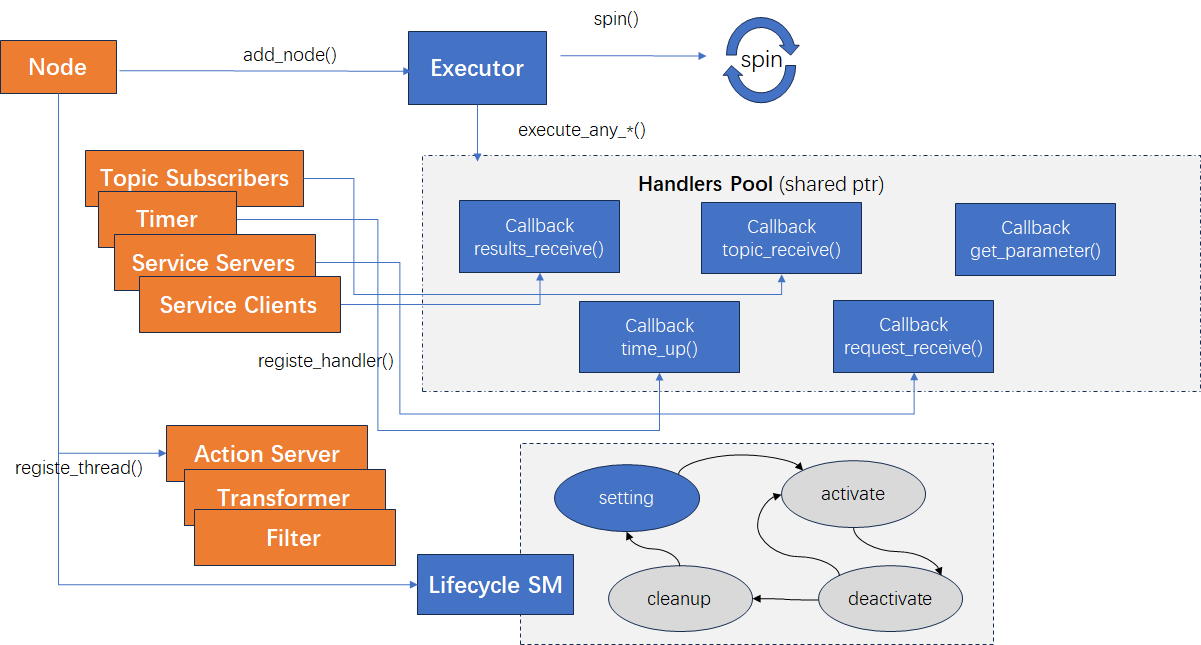
\includegraphics[width=15cm]{ros_node_setup.png}
    \caption{ROS节点内部模型, 初始阶段}
    \label{pic:rns}
\end{figure}

\textbf{ROS 节点释放}

当ROS2系统的节点将释放时,节点的生命周期状态机会从 activate 状态转换为 deactivate 状态,
此状态仅用于让节点完成必要的最后工作,如完成正在处理的数据传输或请求,然后进入非活跃状态。

紧接着,节点生命周期状态机转为 cleanup 状态,见图\ref{pic:rnc},调用 \texttt{cleanup()} 回调函数来释放节点
拥有的资源,这包括所有回调函数(callback handlers),如和话题订阅、定时器、服务等回调
函数。然后清理节点所打开的文件,断开网络连接,释放ROS2上下文,最终释放内存。

\begin{figure}[h]
    \centering
    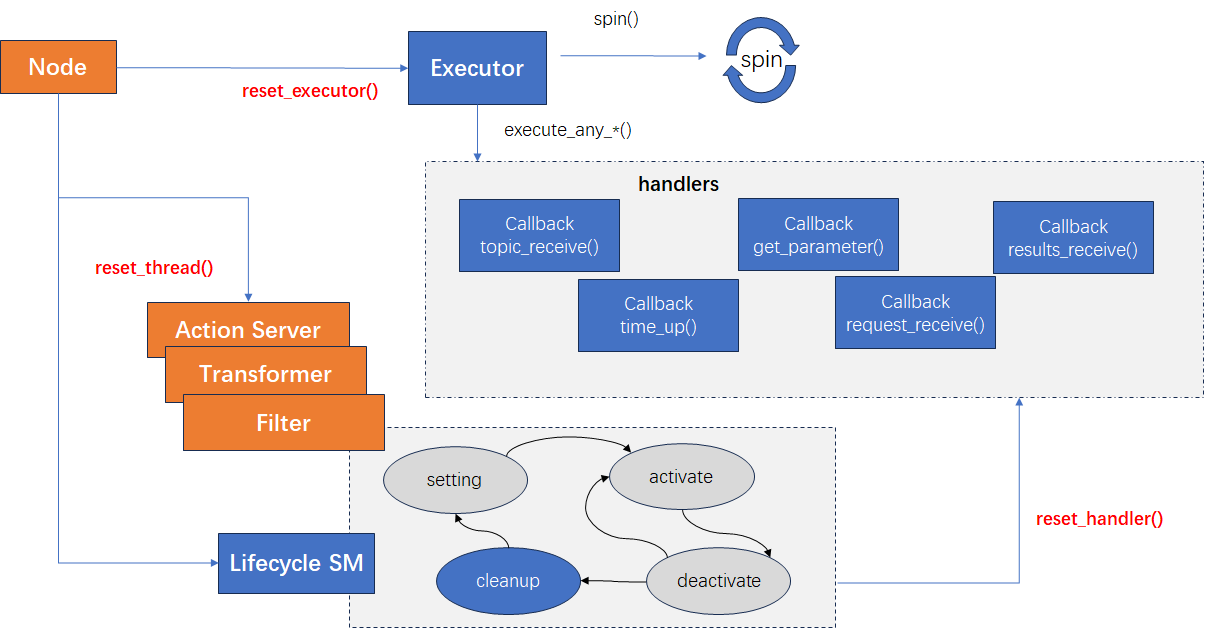
\includegraphics[width=15cm]{ros_node_cleanup.png}
    \caption{ROS节点内部模型, 释放阶段}
    \label{pic:rnc}
\end{figure}

\textbf{ROS 通信机制}

为了适应机器人系统中复杂的通信需求,ROS2设计了一套专用的通信模型。其基础为“发布、订阅“模型,支持节点间的异步数据交换。
该机制允许ROS2系统内的节点(Node)独立地发布(Publish)和订阅(Subscribe)消息,而不需要彼此之间的直接连接或相互了解。
这种设计显著提高了系统的灵活性和扩展性,因为它允许任何数量的发布者和订阅者存在于同一个话题上,从而实现了高效的多对多通信。

在ROS 2的架构中,每个节点可以根据其功能需求,声明为发布者或订阅者,类似图 \ref{pic:rmp},或同时充当这两种角色。
发布者负责生成并发布特定类型的消息到一个命名的话题上,而订阅者则监听这个话题,接收并处理传入的消息。
监听到并处理消息时,使用的是订阅该话题时传入的回调函数来自动处理,订阅者不必同步阻塞就能等待处理订阅消息。
话题本质上是一个数据通道,它通过唯一的名称标识,确保消息的传递和接收的一致性。
每个话题都与一个明确的消息类型相关联,这个消息类型使用YAML格式定义各字段的静态变量类型,从而定义了该话题传输数据的结构。

此通信机制的一个核心优点是其异步性,使得发布者和订阅者可以独立地操作,增加了处理并发消息的能力。
此外,由于发布者和订阅者之间的解耦,系统组件可以被设计得更为模块化,易于开发和维护。
例如,在自动驾驶的应用场景中,激光雷达传感器节点可以发布其测量到的数据到话题 \textbackslash scan,而负责建图和规划路径的节点
则通过订阅该话题来实时获取雷达信息,从而完成最终决策。


\begin{figure}[h]
    \centering
    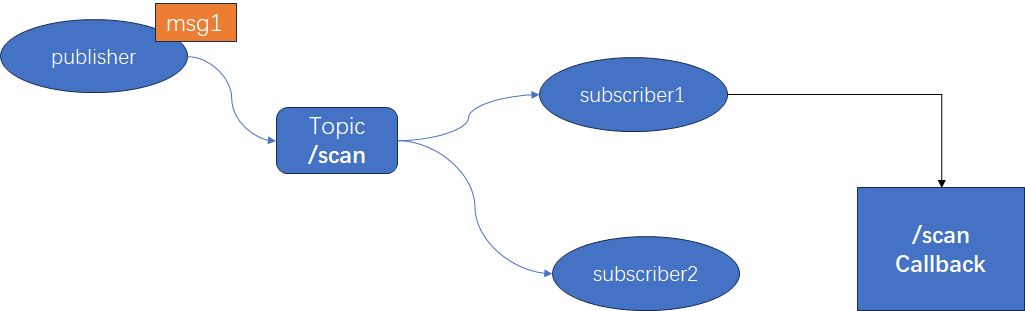
\includegraphics[width=13cm]{ros_msg_passing.png}
    \caption{ROS话题通信机制}
    \label{pic:rmp}
\end{figure}
%@author: yjw

\subsection{关键设计}
\setParDis %设置段间距为 0
%author: yjw, 2024-4-1
%\subsection{关键设计}
\subsection{系统需求分析}
\setParDis %设置段间距为 0
%@author: wkt
\begin{enumerate}
  \item 高覆盖率
  \item 高效性快速收敛
  \item 可拓展性
  \item 准确性高
\end{enumerate}
本项目核心目标是将自动模糊测试(Fuzzing)框架迁移到ROS2系统上,并且针对ROS2特性对测试效率做出改进提升。
具体而言,我们试图寻找更多可能的程序输入口,使测试覆盖的输入可能性尽可能多;尝试构造质量尽可能高的初始种子;
寻找更多反馈信息,用于监控被测程序(即ROS2节点)的内部状态,以更高效地指导对输入的变异;
尝试模拟更多ROS2执行环境,模拟程序可能遇到的各种实际情况。

\subsubsection{多维度输入}
\subsubsection{程序插桩}
\subsubsection{测试加速}


最终,给出本项目的核心框架如图\ref{pic:off}。

\begin{figure}[h]
    \centering
    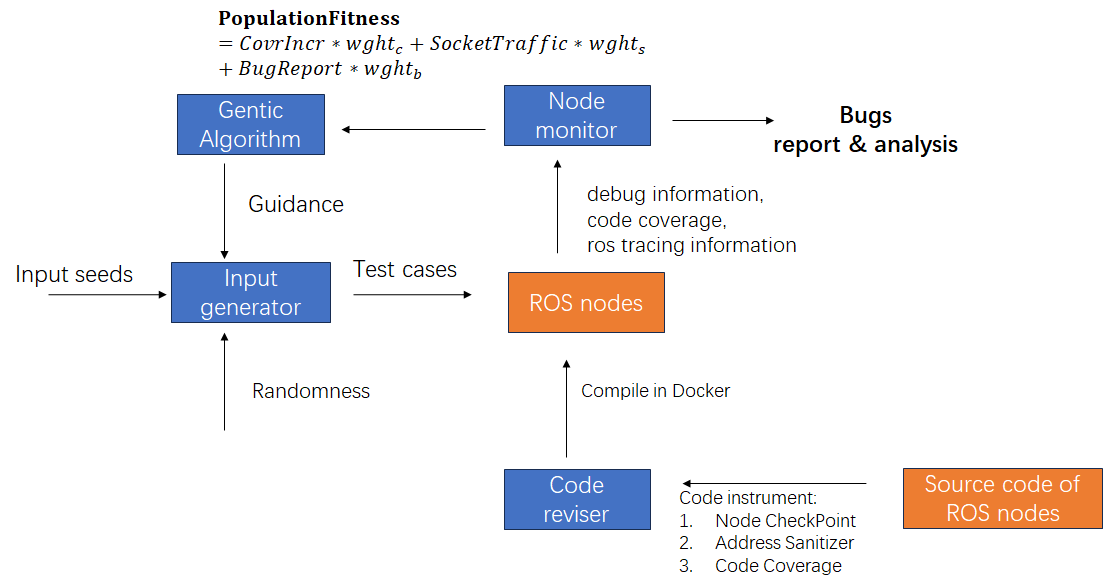
\includegraphics[width=14cm]{our_fuzz_framework.png}
    \caption{本项目实现的Fuzz框架}
    \label{pic:off}
\end{figure}

\subsubsection{测试环境}
%@author: yjw

\section{作品测试与成果分析}
\setParDis %设置段间距为 0
%@author: wkt
\subsection{测试环境介绍}
\setParDis %设置段间距为 0
\subsection{测试成果与漏洞统计}
\setParDis %设置段间距为 0
\subsection{ROS漏洞实例分析}
\setParDis %设置段间距为 0
相关讨论可见GitHub问题 \href{https://github.com/ros-planning/navigation2/issues/4177}{Issue\#4177},提出了ROS 2通信机制中的一个潜在的缓冲区溢出问题。

\begin{lstlisting}[language=]
ros2 topic pub /map nav_msgs/msg/OccupancyGrid "
header:
  stamp:
    sec: 0
    nanosec: 0
  frame_id: map
info:
  map_load_time:
    sec: 0
    nanosec: 0
  resolution: 0.05000000074505806
  width: 2
  height: 2
  origin:
    position:
      x: -10.0
      y: -10.0
      z: 0.0
    orientation:
      x: 0.0
      y: 0.0
      z: 0.0
      w: 1.0
data: [-1, ] " <- buffer overflow
\end{lstlisting}

当\texttt{size\_x\_}和\texttt{size\_y\_}大于数组\texttt{data}大小时,就会导致访问越界(SEGV)。初始化时和接收到\texttt{/map}消息时触发此问题,展示了危险的代码实践。

\begin{lstlisting}[language=cpp]
// create the costmap
costmap_ = new unsigned char[size_x_ * size_y_];

for (unsigned int it = 0; it < size_x_ * size_y_; it++) {
  data = map.data[it]; // <- SEGV
  if (data == nav2_util::OCC_GRID_UNKNOWN) {
    costmap_[it] = NO_INFORMATION;
  } else {
    ...
  }
}
\end{lstlisting}

相关问题和解决方案还包括GitHub \href{https://github.com/ros-planning/navigation2/pull/3958}{PR\#3972}, \href{https://github.com/ros-planning/navigation2/pull/3958}{PR\#3958}, \href{https://github.com/ros-planning/navigation2/issues/3940}{Issue\#3940}, 揭示了并发bug,并通过两个PullRequest得到解决,节省了大量不必要的检查。

最后,讨论了ROS 2节点退出机制可能出现的并发问题,详见 \href{https://github.com/ros-planning/navigation2/issues/4175}{Issue\#4175}, \href{https://github.com/ros-planning/navigation2/pull/4180}{PR\#4180}, \href{https://github.com/ros-planning/navigation2/issues/4166}{Issue\#4166}, \href{https://github.com/ros-planning/navigation2/pull/4176}{Pull\#4176}, 和 \href{https://github.com/ros2/rclcpp/issues/2447}{RclCpp Issue\#2447}。

\subsection{实例分析}
\setParDis %设置段间距为 0
\subsection{与同类技术对比}
\setParDis %设置段间距为 0

\section{创新型说明与前景分析}
\setParDis %设置段间距为 0
%@author: jfb
\subsection{创新性说明}
\setParDis %设置段间距为 0
\begin{enumerate}
  \item 创新地将模糊测试技术迁移
  \item 创新测试方法,高效性
\end{enumerate}

\subsection{前景分析}
\setParDis %设置段间距为 0
\begin{enumerate}
  \item 创新维度
  \item 团队维度
  \item 商业维度
  \item 就业维度
  \item 社会服务
\end{enumerate}

\section*{结论}% section*生成无标号章节
\addcontentsline{toc}{section}{结论} % 将无标号章节添加至目录
%@author: jfb
傻逼冯如杯

%注意: 文件大小不超过5M。%

\end{spacing}
%%%%%%%%%%%%%%%%%%%%引用部分
\newpage

% XSP 2023/3/16: bib支持不全,暂时改为手动
\section*{参考文献} % section*生成无标号章节题目
\addcontentsline{toc}{section}{参考文献} % 将无标号章节添加至目录
% 著作: [序号]作者.书名[标识码].出版地:出版社,出版年.
[1]张志建.严复思想研究[M].桂林:广西师范大学出版社,1989. 

% 译著: [序号]国名或地区(用圆括号)原作者.书名[标识码].译者.出版地:出版社,出版年.
[2](英)霭理士.性心理学[M].潘光旦译.北京:商务印书馆,1997.

% 古典文献 文史古籍类引文后加序号,再加圆括号,内加注书名、篇名

% 论文集: [序号]编者.书名[标识码].出版地:出版社,出版年.
[3]伍蠡甫.西方论文选(下册)[C].上海:上海译文出版社,1979.

% 期刊文章: [序号]作者.篇名[标识码].刊名,年,(期).
[4]叶朗.《红楼梦》的意蕴[J].北京大学学报(哲学社会科学版),1989,(2)

% 报纸文章: [序号]作者.篇名[标识码].报纸名,出版日期(版次)
[5]谢希德.创造学习的新思路[N].人民日报,1998-12-25(10)

% 外文文献: 要求外文文献所表达的信息和中文文献一样多,但文献类型标识码可以不标出。
[6]Mansfeld, R.S. \& Busse. \textit{T.V. The Psychology of creativity and discovery}, Chinago:
NelsonHall, 1981




% \begingroup
% \setstretch{2.0}    %行距2
% \setlength{\bibsep}{0pt}    %段前段后0
% \begin{adjustwidth}{0.42cm}{0.42cm} %左右缩进0.42cm
% \bibliography{references}
% \end{adjustwidth}
% \endgroup

\end{document}
